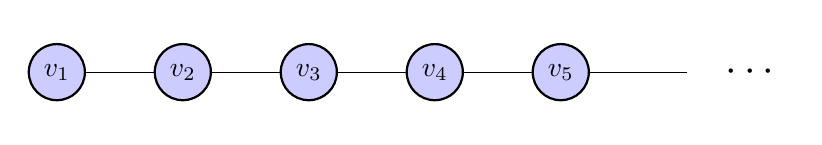
\begin{tikzpicture}
  [scale=.8,auto=left,every node/.style={circle,fill=blue!20,draw=black,thick}]
  \node (n1) at (0,0) {$v_1$};
  \node (n2) at (2,0)  {$v_2$};
  \node (n3) at (4,0)  {$v_3$};
  \node (n4) at (6,0) {$v_4$};
  \node (n5) at (8,0)  {$v_5$};

  \foreach \from/\to in {n1/n2,n2/n3, n3/n4, n4/n5}
    \draw (\from) -- (\to);

   %Flecha de (n5) a un nodo invisible en (10,0)   
   \draw (n5) -- (10,0);
   
   %Etiqueta de puntos suspensivos
   \node[draw=none, fill=none, scale=1.5] at (11,0) {$\cdots$};
   % Etiqueta G_1 debajo del grafo
%   \node[draw=none, fill=none, scale=1.5] at (6,-1.5) {$G_5$};
\end{tikzpicture}
